\documentclass{article}

\usepackage[utf8]{inputenc}
\usepackage{stmaryrd}
\usepackage[french]{babel}
\usepackage{amsmath}
\usepackage{graphicx}

\title{Résolution d'équations différentielles à l'aide de réseaux de neurones}
\author{Matthieu Carreau, encadré par Stam Nicolis et Pascal Thibaudeau}
\date{Juillet 2022}

\begin{document}

\maketitle


\section{Présentations de différentes approches pour la résolution d'une équation différentielle d'ordre 1}
On cherche à tester nos méthodes sur l'équation différentielle suivante, pour $x\in [0,1]$ :

\begin{equation}
\left\{
    \begin{array}{ll}
        \frac{d\Psi}{dx} + cos(2\pi x) = 0 \\
        \Psi(0) = A
    
    \end{array}
\right.
\label{eq:equa dif}
\end{equation}

Cette équation avec condition initiale admet une unique solution analytique :
\begin{equation}
    {\Psi}(x) = A - \frac{1}{2\pi}sin(2\pi x)
\label{eq:solution analytique}
\end{equation}

\subsection{Recherche de solutions en série de Fourier}

On cherche des solutions numériques approchées sous la forme de séries de Fourier tronquées avec $M$ harmoniques :

\begin{equation}
\left\{
    \begin{array}{ll}
        \Tilde{\Psi}(x) = A + {\mathcal{N}}(x,P) \\
        {\mathcal{N}}(x,P) = \sum_{m=1}^{M} A_m sin(2\pi m x) 
    \end{array}
\right.
\label{eq:solution Fourier}
\end{equation}

$P$ représente les coefficients $(A_m)_{m\in \llbracket 1,M \rrbracket}$ qui sont les paramètres à ajuster.
On cherche à obtenir la solution analytique, i.e $\forall m \in\llbracket 1,M \rrbracket, A_m = -\frac{1}{2\pi}\delta _1 ^m $.

On définit une fonction d'erreur pour ces solutions potentielles, en s'interressant aux $N$ points suivants : $\forall i \in\llbracket 1,N \rrbracket, x_i = \frac{i}{N-1} $

\begin{equation}
    E = \frac{1}{2}\sum_{i=1}^{N}(\sum_{m=1}^{M} 2\pi m A_m cos(2\pi m x_i)+cos(2\pi x_i))^2 
\label{eq:fonction d'erreur}
\end{equation}

On calcule alors la dérivée partielle de cette erreur par rapport à chaque paramètre $A_l$ :

\begin{equation}
    \frac{\partial E}{\partial A_l} = 
    \sum_{i=1}^{N}(\sum_{m=1}^{M} 2\pi m A_m cos(2\pi m x_i)+cos(2\pi x_i))
    2\pi l cos(2\pi l x_i)
\label{eq:gradient}
\end{equation}

Les deux méthodes suivantes ont pour objectif de trouver les coefficient $(A_m)_{m\in \llbracket 1,M \rrbracket}$ qui minimisent $E$.

\subsubsection{Première méthode : inversion d'un système linéaire}

On cherche à résoudre le système linéaire donné par : 
$\forall m \in\llbracket 1,M \rrbracket, \frac{\partial E}{\partial A_l} = 0$, on définit pour cela les matrices suivantes :



\begin{equation}
    \mathcal{M} = (r_{m,l})_{(m,l)\in \llbracket 1, M\rrbracket ^2}, 
    \Vec{A} = \begin{pmatrix}
                A_1 \\
                A_2 \\
                \vdots \\
                A_M
              \end{pmatrix}, 
    \Vec{b} = \begin{pmatrix}
                b_1 \\
                b_2 \\
                \vdots \\
                b_M
              \end{pmatrix}
\label{eq:définition notation}
\end{equation}

\begin{equation}
\forall (m,l) \in \llbracket 1, N\rrbracket ^2,
\left\{
    \begin{array}{ll}
        r_{m,l} = 2\pi ml \sum_{i=1}^{N}cos(2\pi mx_i)cos(2\pi lx_i) \\
        b_l = -l\sum_{i=1}^{N}cos(2\pi x_i)cos(2\pi lx_i)
    \end{array}
\right.
\label{eq:définition coefficients}
\end{equation}

On résoud le système en écrivant l'équation matricielle le représentant :

\begin{equation}
    \mathcal{M} \Vec{A} = \Vec{b} \Leftrightarrow \Vec{A} = \mathcal{M}^{-1}\Vec{b} 
\label{eq:équation matricielle}
\end{equation}

(Attention pour  certains paramètres comme $(M=5, N=10)$, $\mathcal{M}$ n'est pas inversible). \\

On initialise l'algorithme avec les paramètres suivants :
$(M=10, N=100)$
On obtient les résultats suivants : \\
$A = [-1.59154943e-01,  4.74338450e-19,  1.08420217e-19,  2.71050543e-20,
2.74438675e-19,  1.05032085e-19,  9.82558219e-20,  5.92923063e-20,
5.42101086e-20,  5.42101086e-20]$ \\
On constate comme attendu que le coefficient $A_1$ est très proche de $-\frac{1}{2\pi}$ (erreur relative de l'ordre de $10^{-16}$), et que les autres coefficients ont une valeur absolue maximale de $1.15 10^{-17}$.
On peut donc valider notre modèle.


\subsubsection{Seconde méthode : descente de gradient}

On définit les paramètres suivants :

\begin{equation}
    \alpha>0, 
    \Vec{A}^{(0)} = \begin{pmatrix}
                A_1^{(0)} \\
                A_2^{(0)} \\
                \vdots \\
                A_M^{(0)}
              \end{pmatrix},
    \Vec{g}^{(0)} = \begin{pmatrix}
                \frac{\partial E^{(0)}}{\partial A_1^{(0)}} \\
                \frac{\partial E^{(0)}}{\partial A_2^{(0)}} \\
                \vdots \\
                \frac{\partial E^{(0)}}{\partial A_M^{(0)}}
              \end{pmatrix},     
\label{eq:définition descente de gradients}
\end{equation}

Puis on calcule itérativement :

\begin{equation}
    \Vec{A}^{(k+1)} = \Vec{A}^{(k)} - \alpha\Vec{g}^{(k)} 
\label{eq:équation récurrence descente gradients}
\end{equation}



On initialise l'algorithme avec les paramètres suivants :
$(M=10, N=100, V_0 = 1, \alpha = 10^{-5})$
On obtient au bout de 10000 itérations les résultats suivants : \\
$A = [-1.59154943e-01,  1.15066541e-17,  7.99406786e-18,  5.64963221e-18,
4.88181580e-18,  3.85811144e-18,  3.46024465e-18,  2.88560910e-18,
2.81846501e-18, 2.43172156e-18]$ \\
On constate comme attendu que le coefficient $A_1$ est très proche de $-\frac{1}{2\pi}$ (erreur relative de l'ordre de $10^{-15}$), et que les autres coefficients ont une valeur absolue maximale de $1.15 10^{-17}$.
On peut donc valider notre modèle.


\subsection{Recherche de solutions à l'aide d'un réseau de neurones}

On cherche à présent à utiliser un réseau de neurones pour approcher la solution de l'équation différentielle. On cherche désormais des solutions approchées sous la forme suivante :

\begin{equation}
\left\{
    \begin{array}{ll}
        \Tilde{\Psi}(x) = A + {\mathcal{N}}(x,P) \\
        {\mathcal{N}}(x,P) = \sum_{j=1}^{H} v_j \sigma(w_jx+b_j)
    \end{array}
\right.
\label{eq:solution NN}
\end{equation}

${\mathcal{N}}(x,P)$ correspond donc à la sortie d'un réseau de neurones dont l'architecture est présentée en figure \ref{fig:NN}, contenant une couche cachée intermèdiaire, qui réalise en sortie une somme pondérée de sigmoïdes, la fonction utilisée est $\forall x \in \mathbf{R}, \sigma(x) = \frac{1}{1+e^{-x}}$. Les paramètres $P$ à ajuster sont désormais les coefficients $(w_j)_{j\in \llbracket 1,H \rrbracket}$, $(b_j)_{j\in \llbracket 1,H \rrbracket}$ et $(v_j)_{j\in \llbracket 1,H \rrbracket}$.

\begin{figure}
\centering
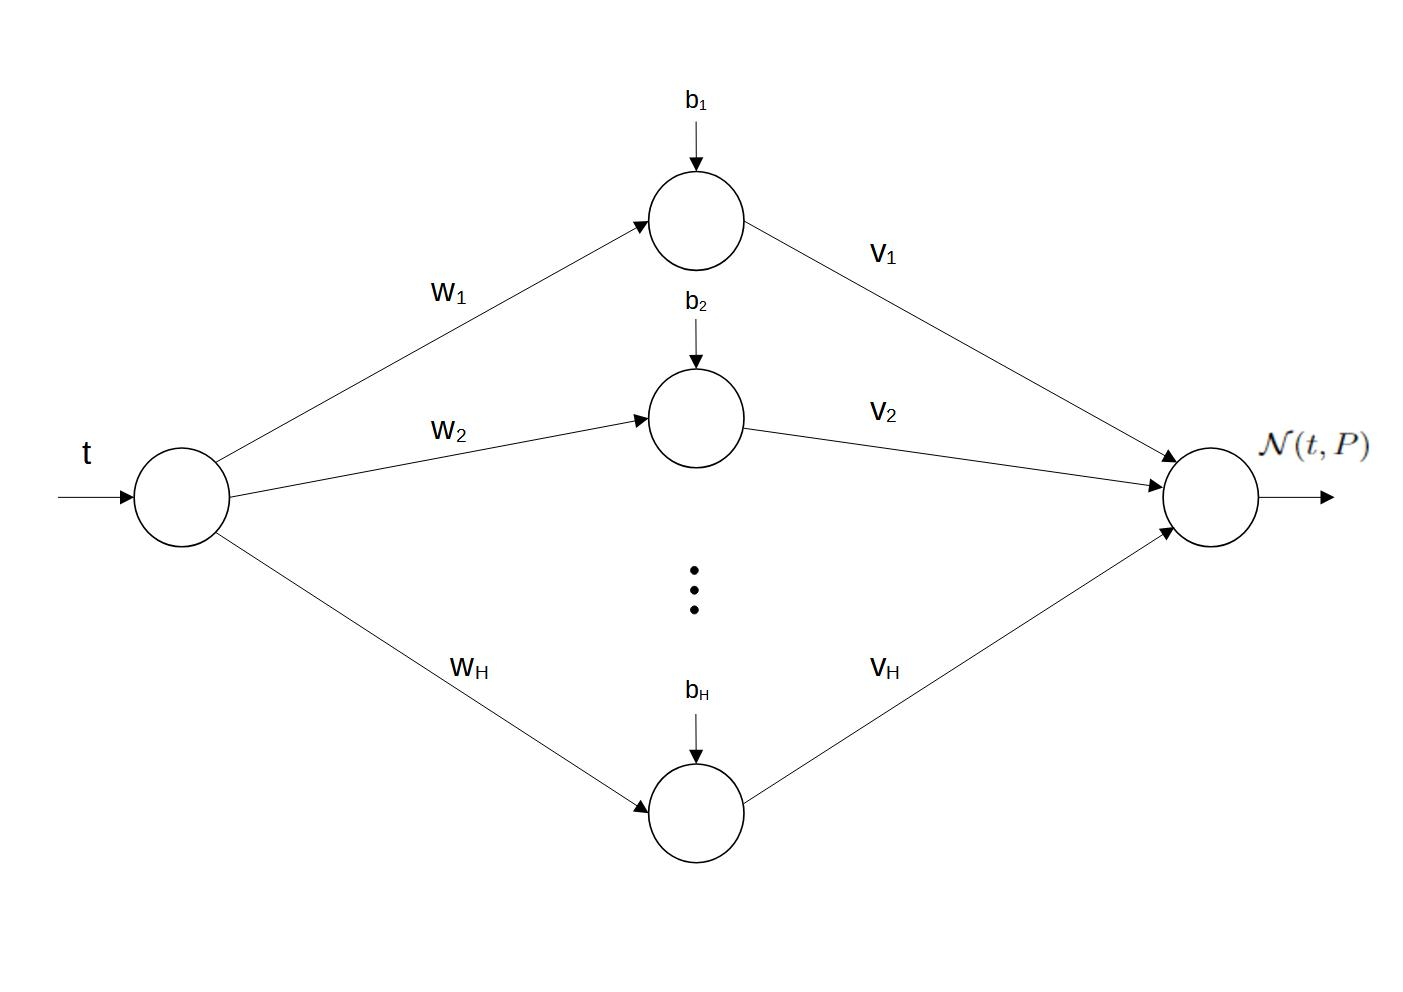
\includegraphics[width=0.8\textwidth]{NN.jpg}
\caption{\label{fig:NN}Réseau de neurones}
\end{figure}

On définit une nouvelle fonction d'erreur, calculée à partir des mêmes $N$ points que précédemment : $\forall i \in\llbracket 1,N \rrbracket, x_i = \frac{i}{N-1} $

\begin{equation}
        E(P) = \sum_{i=1}^{N} (\frac{d\Tilde{\Psi}}{dx}(x_i) + cos(2\pi x))^2
\label{eq:erreur NN}
\end{equation}

On calcule ensuite les expressions analytiques des dérivées partielles de $E(P)$ par rapport à chaque paramètre ajustable, puis on cherche à minimiser cette erreur à l'aide de l'algorithme de descente de gradients.

\subsubsection{Résultats obtenus}
On initialise l'algorithme avec les paramètres suivants :
$(H=4, N=20)$
On obtient une erreur de $1,2.10^{-2}$ et une estimation visible en figure \ref{fig:resultat_NN}. Cela permet de valider notre modèle sur l'étude à une dimension.

\begin{figure}
\centering
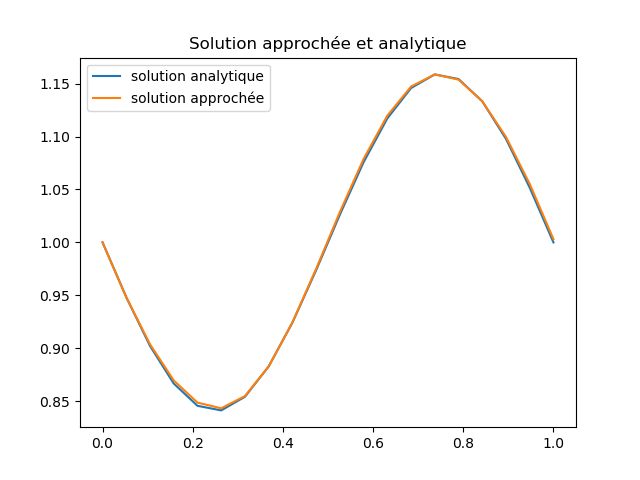
\includegraphics[width=0.8\textwidth]{resultat_NN.png}
\caption{\label{fig:resultat_NN}estimation de la solution par un réseau de neurones}
\end{figure}


\section{Etude du cas de deux équations d'ordre 1 couplées, représentant un mouvement de précession}
On s'intéresse désormais au problème de la précession d'un moment magnétique dans un champ magnétique constant. On le modélise par les équations suivantes pour $t\in [0,1]$ :

\begin{equation}
\left\{
    \begin{array}{ll}
        \frac{dv_x}{dt} = \omega v_y \\
        \frac{dv_y}{dt} = -\omega v_x
    \end{array}
\right.
\left\{
    \begin{array}{ll}
        v_x(0) = V_0 \\
        v_y(0) = 0
    \end{array}
\right.
\label{eq:équations couplées}
\end{equation}

Ce problème admet une unique solution analytique :
\begin{equation}
\left\{
    \begin{array}{ll}
        v_x(t) = V_0 cos(2\omega t) \\
        v_y(t) = -V_0 sin(2\omega t)
    \end{array}
\right.
\label{eq:solution analytique couplée}
\end{equation}

\subsection{Recherche des solutions en séries de Fourier}
On cherche des solutions numériques approchées sous la forme de séries de Fourier tronquées avec $M$ harmoniques, en posant la forme suivante :

\begin{equation}
\left\{
    \begin{array}{ll}
        \Tilde{v}_x(t) = V_0 + \sum_{m=1}^{M} A_m (cos(\omega m t)-1) + B_m sin(\omega m t) \\
        \Tilde{v}_y(t) = \sum_{m=1}^{M} -A_m sin(\omega m t) + B_m (cos(\omega m t)-1)
    \end{array}
\right.
\label{eq:solution Fourier couplée}
\end{equation}

Les coefficients $(A_m)_{m\in \llbracket 1,M \rrbracket}$ et $(B_m)_{m\in \llbracket 0,M \rrbracket}$ sont les paramètres à ajuster.
On cherche à obtenir la solution analytique, i.e $\forall m \in\llbracket 0,M \rrbracket, A_m = \delta _1 ^m $ et $\forall m \in\llbracket 1,M \rrbracket, B_m = 0 $. On remarque que le coefficient $A_0$ n'a aucune influence.

On définit une fonction d'erreur pour ces solutions potentielles, en s'interressant aux $N$ points suivants : $\forall i \in\llbracket 1,N \rrbracket, t_i = \frac{i}{N-1} $ :

\begin{equation}
        E(P) = \sum_{i=1}^{N} (\frac{d\Tilde{v}_x}{dt}(t_i) - \omega \Tilde{v}_y(t_i))^2 + (\frac{d\Tilde{v}_y}{dt}(t_i) + \omega \Tilde{v}_x(t_i))^2
\label{eq:erreur descente gradient couplées}
\end{equation}

On utilise ensuite la méthode de descente de gradients définie précédemment, en calculant les dérivées partielles suivantes :
$(\frac{\partial E}{\partial A_l}, \frac{\partial E}{\partial B_l})_{l \in \llbracket 1,M \rrbracket}$

\subsubsection{Résultats obtenus}
On initialise l'algorithme avec les paramètres suivants :
$(M=10, N=100, V_0 = 1, \omega = 2\pi, \alpha = 10^{-6})$
On obtient au bout de 10000 itérations les résultats suivants : \\
$A = [1.00000255e+00, -1.23919994e-06, -2.20679520e-07, -9.12537244e-08,
-4.93048945e-08, -3.05670278e-08, -2.06219718e-08, -1.47337251e-08,
-1.09721848e-08, -8.43076573e-09], \\
B = [-6.59235880e-07,  3.20274560e-07,  5.70352161e-08,  2.35847707e-08,
1.27429827e-08,  7.90013061e-09,  5.32980412e-09,  3.80797092e-09,
2.83579070e-09,  2.17895410e-09]$ \\
On constate comme attendu que le coefficient $A_0$ est très proche de 1 (erreur relative inférieure de $2.55 10^{-6}$), et que les autres coefficients ont une valeur absolue maximale de $1.24 10^{-6}$.
On peut donc valider notre modèle.

\end{document}

